\chapter{基于注意力机制的地理知识库问答模型}
基于注意力机制的地理知识库问答模型是指运用基于注意力机制的双向循环神经网络,对用户提出的地理问题,以及将从知识库搜索出的问题答案三元组进行表示的模型。本章先介绍本文问答模型的核心算法,这些核心算法是对问题、答案的表示模型,包括RNN、LSTM、Bi-LSTM、Attention Based Bi-LSTM;然后介绍模型的训练方法;最后介绍模型实验,包括实验目的、实验参数设置、实验数据集构建、实验评价指标和实验结果及分析。

\section{模型核心算法}
本节讲述如何将地理问题和候选答案文本序列表示成词向量(word embedding)形式。本文表示地理和候选答案的基础模型为循环神经网络( Recurrent Neural Network,RNN),本节介绍使用RNN的变种LSTM模型来表示地理问题和答案,先介绍RNN表示序列数据的原理,后依次介绍使用基于基本的LSTM表示问题、答案,基于Bi-LSTM来表示问题答案和基于Attention的Bi-LSTM表示答案。

\subsection{RNN表示序列数据原理}
RNN的网络结构如图\ref{fig:rnn_structure}所示,图左边部分表示RNN的循环结构图,RNN的主体结构单元A处理来自当前时刻的输入$x_{i}$和上一时刻A输出的隐含状态。图的右边是左边图的展开形式。RNN中每一层不仅输出$h_{i}$到下一层,而且同时还输出一个隐含状态(hidden state),该隐含状态表示当前层和之前所有层保存的信息,可以形象化地理解为当前到之前层的所有信息的综合记忆,下一层可以利用上一层输出的隐含状态信息。因此,RNN此网络特征结构也使其擅长处理前后有依赖关系的序列数据。

\begin{figure}[!htb]
	\centering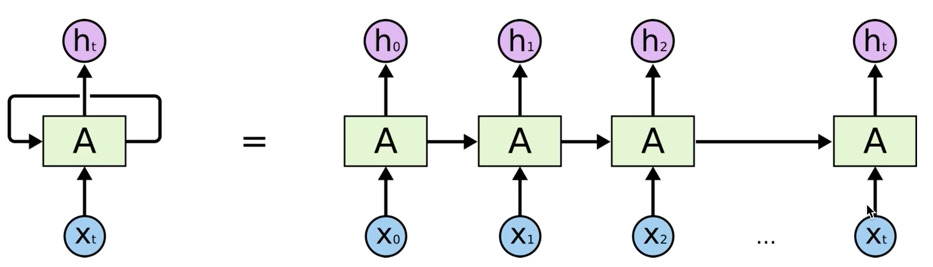
\includegraphics[height=3cm]{resource/rnn_structure}
	\caption{RNN网络结构}
	\label{fig:rnn_structure}
\end{figure}

\subsection{基于LSTM的问题、答案表示}
在实际中,对于文本序列来说,循环神经网络较难捕捉两个时刻距离较大的文本元素(字或词)之间的依赖关系。LSTM 是 RNN 的变种之一,是一种常用的门控循环神经网络,可以解决 RNN 中的梯度消失、梯度爆炸问题。本文实现的 LSTM 为基于Graves\cite{Graves}等人改进的 LSTM。给定输入问句,令其序列 \textbf{x}=\{x(1),x(2),…x(n)\},其中 x(t)为问句中每个词的 d 维词向量表示,隐藏单元向量$\textbf{$h_{t}$}$遵循如下更新方式:

$$
i_t = \sigma(\textbf{W}_{ix}\textbf{x}(t) + \textbf{W}_{ih}\textbf{h}(t - 1) + \textbf{b}_i)
\eqno(3)
$$
$$
f_t = \sigma(\textbf{W}_{fx}\textbf{x}(t) + \textbf{W}_{fh}\textbf{h}(t - 1) + \textbf{b}_f)
\eqno(4)
$$
$$
o_t = \sigma(\textbf{W}_{ox}\textbf{x}(t) + \textbf{W}_{oh}\textbf{h}(t - 1) + \textbf{b}_o)
\eqno(5)
$$
$$
\tilde{C}_t = \tanh(\textbf{W}_{cx}\textbf{x}(t) + \textbf{W}_{ch}\textbf{h}(t - 1) + \textbf{b}_c)
\eqno(6)
$$
$$
C_t = i_t \odot \tilde{C}_t + f_t \odot C_{t-1}
\eqno(7)
$$
$$
\textbf{h}_t = o_t \odot \tanh (C_t)
\eqno(8)
$$

此 LSTM结构通过三个门,输入门 i、输出门 o、遗忘门 f 和记忆单元 c 来控制该时刻前的历史信息是否需要记忆、是否需要更新,从而更好的对历史信息进行保存,供下一时刻使用。公式中的$\textbf{W}_{ix}$、 $\textbf{W}_{ih}$、$\textbf{W}_{fx}$、$\textbf{W}_{fh}$、$\textbf{W}_{ox}$、$\textbf{W}_{oh}$、$\textbf{W}_{cx}$、$\textbf{W}_{ch}$、$\textbf{W}_{cx}$、$\textbf{W}_{ch}$是可学习的权重参数,$\textbf{b}_i$、$\textbf{b}_f$、$\textbf{b}_o$、$\textbf{b}_c$是可学习的偏移参数,$\textbf{h}(t - 1)$为上一时刻的隐含状态输出值,函数σ为sigmoid激活函数,tanh为双曲正切函数作为激活函数,$\tilde{C}_t$表示长短期记忆中的候选记忆单元值,$C_{t-1}$为上一时刻的记忆单元值,$C_t$为当前时刻的记忆单元值,$\odot$为按元素乘法符。

本文首先通过分词将问题转化为词序列,此处记作 $\textbf{q}$ = \{x(1), x(2),…x(n)\}, x(i)表示问题词序列第 i个词, 然后查询词向量矩阵(初始为根据中文维基百科训练得到)获得每个词的初始词向量,最后将序列的词向量输入到上述 LSTM 模型,遵循其更新法进行训练,得到序列最终的词向量。

\subsection{基于Bi-LSTM的问题、答案表示}
单向 LSTM 模型只考虑当前输入之前的信息,没有考虑其输入之后的信息,往往一个词的含义需要综合考虑此词的前后两部分词信息。因此,本文使用 Bi-LSTM,综合考虑当前输入的前向和后向信息, 隐藏单元为前向$\overrightarrow{h_t}$、后向单元$ \overleftarrow{h_t}$相连接,如公式(7 )所示:
$$
h_t = (\overrightarrow{h_t}, \overleftarrow{h_t})
\eqno(9)
$$
因此,本文基于 Bi-LSTM 的问答模型可以表示为图\ref{fig:qa_bi_lstm}问答模型所示。 
\begin{figure}[!htb]
	\centering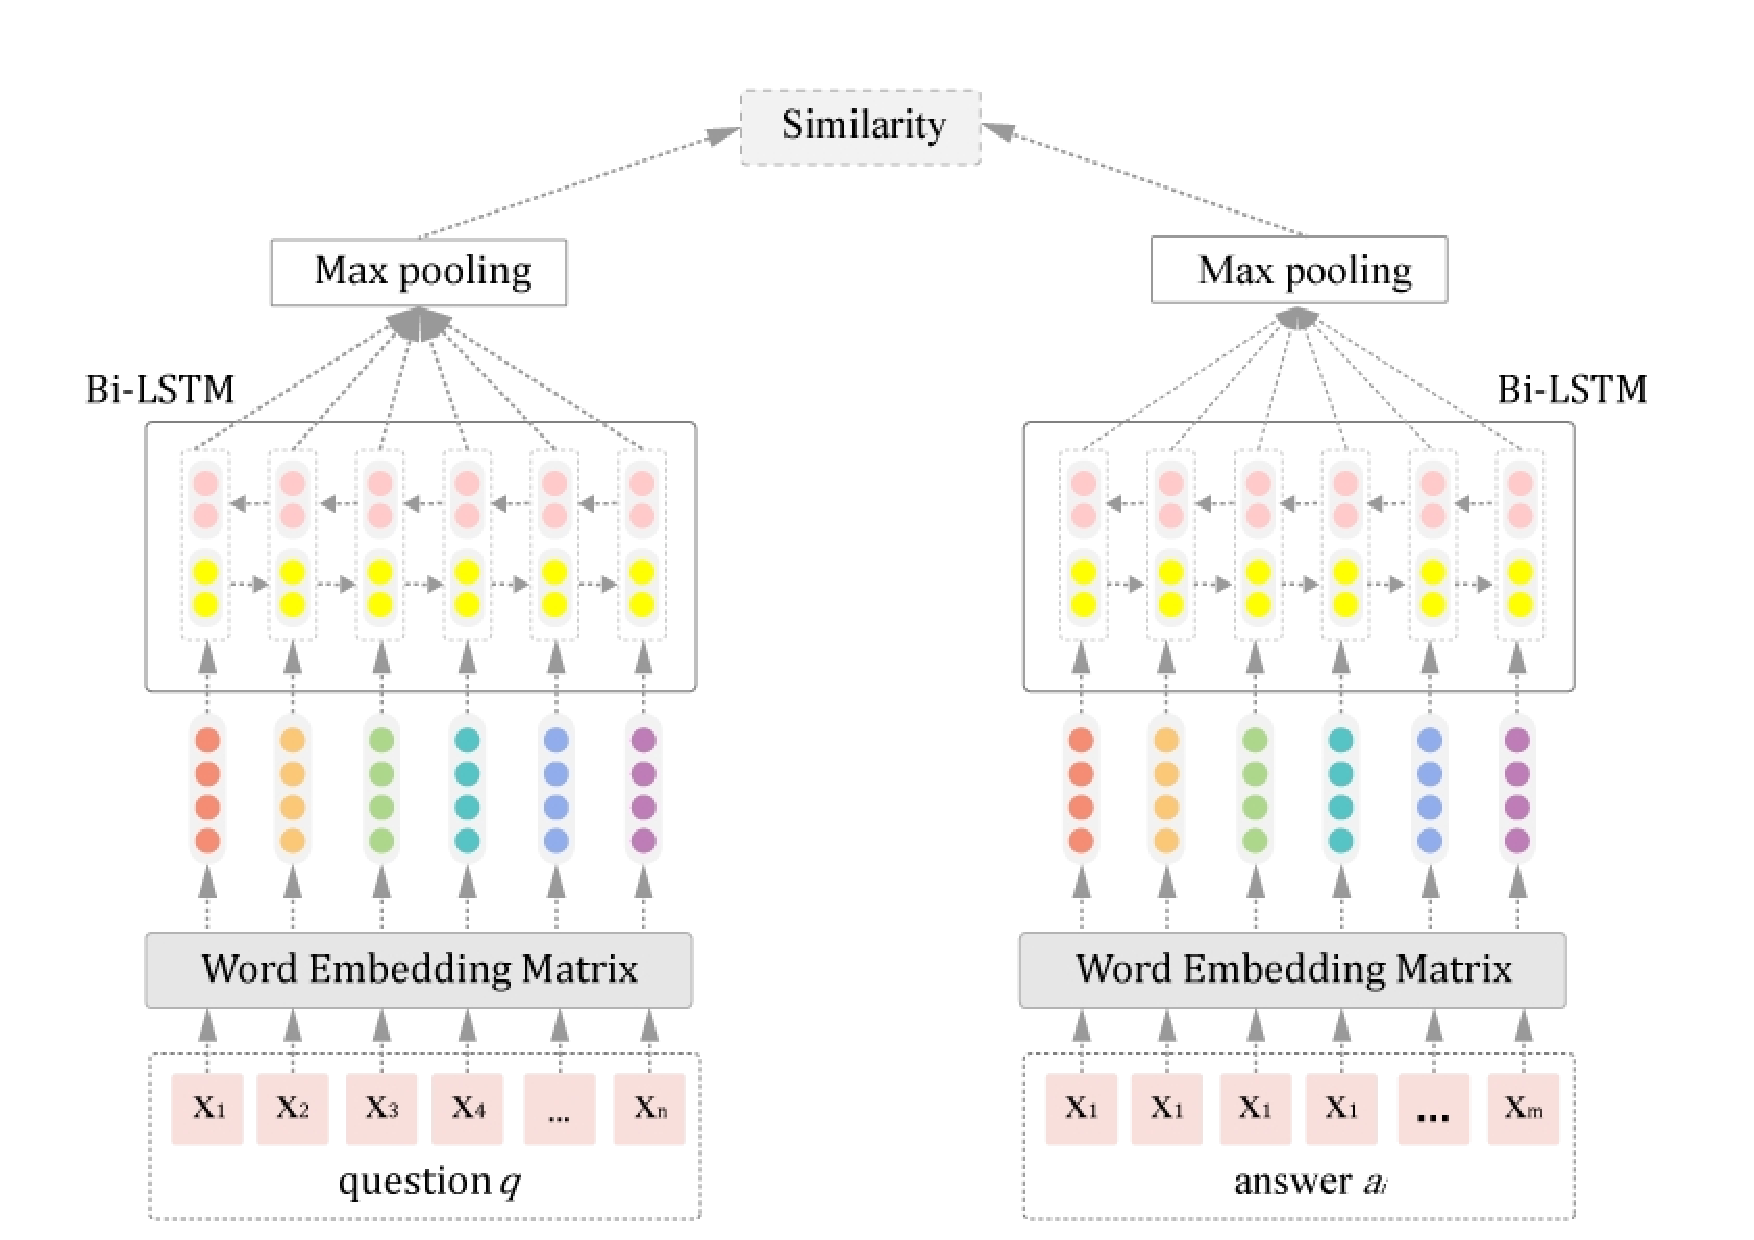
\includegraphics[height=8cm]{resource/qa_bi_lstm_1}
	\caption{基于Bi-LSTM的问题、答案表示模型}
	\label{fig:qa_bi_lstm}
\end{figure}

该问答模型首先生成问题、答案词序列的初始词向量, 然后输入到 Bi-LSTM 网络进入训练,得到问题和答案的最终向量表示, 最后词向量做 max pooling 后通过余弦相似性计算问题、答案向量矩阵的相似性。实验设置问题、答案的 Bi-LSTM 网 络共享参数, Feng\cite{Feng}等人的研究表明两个网络共享 参数较两个网络拥有各自不同参数性能更优。

\subsection{基于注意力机制的答案表示}
与上述模型单独对问题和答案进行表示不同,此节使用一种基本的注意力机制模型,答案中每个词的向量生成均依赖问题,通过动态地将答案中更多的有效信息与问题相应关键信息对齐,可以更好的表示答案与问题之间的依赖关系。 该注意力机制已在许多自
然语言处理任务上取得不错效果,如机器翻译、事实型问答、句子摘要等。

图3.6为本文基于注意力机制的答案表示模型,模型使用词级别的注意力,如图3.6中描述,在答案端Bi-LSTM 网络输出进入 max pooling 层之前,每个输出会乘以一个基于问题的 Attention 值。 时间 t 时刻, 令答案端的 Bi-LSTM 输出向量为$\textbf{h}_{a}(t)$ ,问题词向量为$\textbf{o}_q$,答案中每个词向量$\tilde{\textbf{h}}_{a}(t)$更新如下:
$$
\textbf{m}_{a,q}(t) = \tanh(\textbf{W}_{am}\textbf{h}_{a}(t) + \textbf{W}_{qm}\textbf{o}_q)
\eqno(10)
$$
$$
s_{a,q}(t) = softmax(\textbf{w}_{sm}\textbf{m}_{a,q}(t))
%s_{a,q}(t) = softmax(\textbf{w}_{sm} \tanh(\textbf{W}_{am}\textbf{h}^{a}_t + \textbf{W}_{qm}\textbf{o}_q))
\eqno(11)
$$
$$
\tilde{\textbf{h}}_{a}(t) = \textbf{\textbf{h}}_{a}(t) s_{a,q}(t)
\eqno(12)
$$

其中,$\textbf{W}_{am}$、$\textbf{W}_{qm}$为注意力机制参数矩阵,$\textbf{w}_{sm}$为注意力机制参数向量。从直观上看, 运用注意力机制表示答案相当于一定程度上将答案中与问题相对应关键词增加权重,给无关词减少权重,使更易于区分正确答案和错误答案。

\begin{figure}[!htb]
	\centering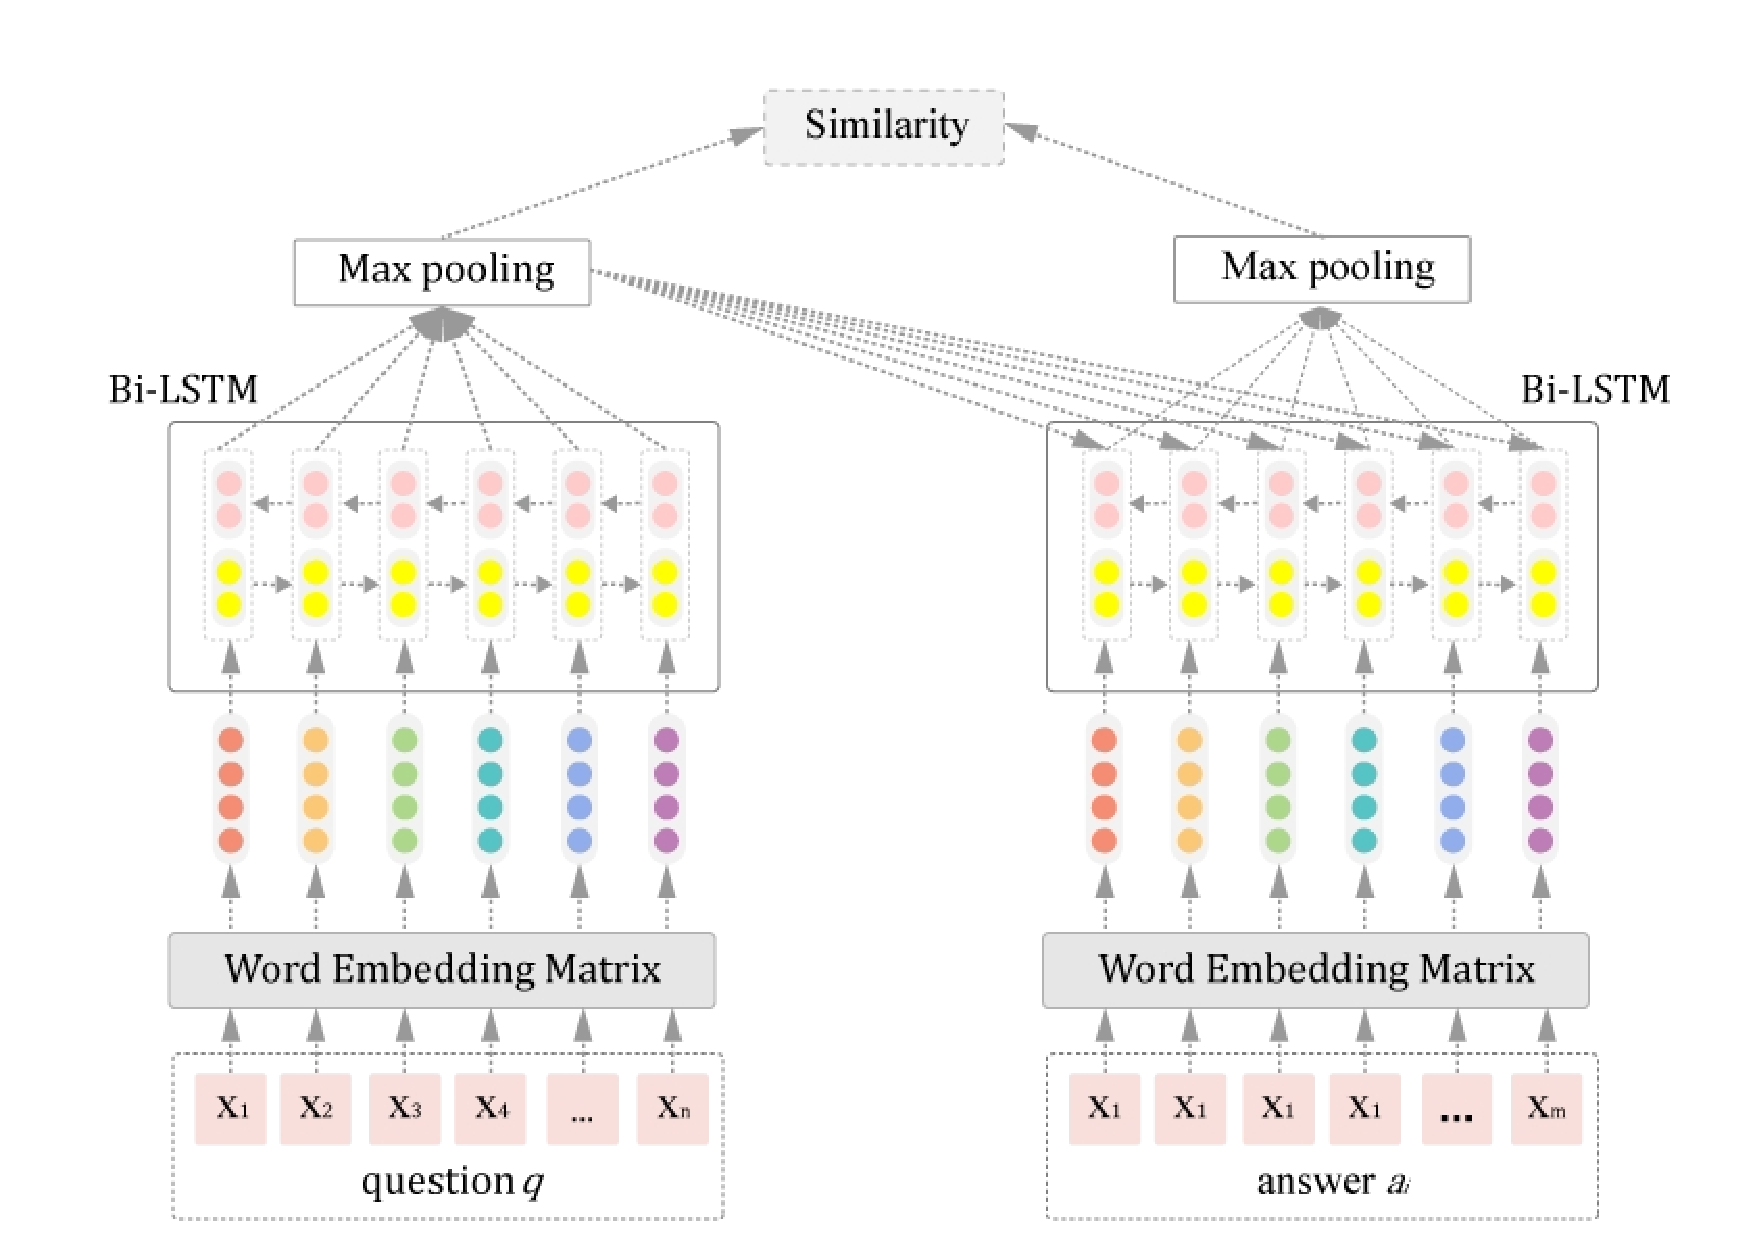
\includegraphics[height=8cm]{resource/qa_attention_1}
	\caption{基于Attention机制的问题、答案表示模型}
	\label{fig:qa_attention}
\end{figure}

\section{模型训练}
本文采取问答常用的训练方式pairwise training\cite{Burges},训练数据形式为(问题、正确答案、错误答案)。对于某个问题,本文选取一个正确答案作为正例,同时选取k个错误答案作为负例,负例的选择一部分来自主题实体的非答案三元组,另一部分随机从其他问题的正确答案中选取。损失函数使用铰链损失函数(hinge loss),如下:
$$
\mathcal{L}(q, a_+, a_-) = max \{0, m - S(q, a_+) + S(q, a_-)\}
\eqno(13)
$$

m为正确答案得分和错误得分差距,S(.)为余弦函数,$a_+$为问题的正确答案,$a_-$为问题的错误答案。目标函数为:

$$
\min \sum_q\frac{1}{|P_q|}\sum_{a_+ \in P_q}\sum_{a_- \in N_q} \mathcal{L}(q, a_+, a_-)
\eqno(14)
$$

其中$|P_q|$为问题q的正确答案个数,$N_q$为问题q的k个错误答案集合。本文采取随机梯度下降(stochastic gradient descent,SGD)学习算法。

\section{实验}
为了评估本文问答模型的性能,本文使用本文构建的地理本体知识库,同时为了解决目前中文地理领域问题缺乏的问题,本文又构建了较大规模的地理问题测试集。本节先介绍实验目的、参数设置,然后介绍实验数据集构建,最后介绍实验结果以及实验分析。

\subsection{实验目的}
本文分别使用LSTM、Bi-LSTM和Attention Based Bi-LSTM模型进行实验,通过对比实验性能指标来证明Attention-Based Bi-LSTM问答模型的有效性。

\subsection{实验参数设置}
实验词向量由word2vec\cite{Mikolov}结合最新的中文维基百科语料训练得到,词向量维度为300。实验采取随机梯度下降优化策略,实验尝试过不同的m值,如0.1、0.2、0.3,最终选择0.1效果较佳。学习率初始值为0.4,每10个epochs下降50$\%$,总共下降4次。剪枝参数max\_grad\_norm设为5,dropout取1.0。实验batch\_size取50,问题负例个数k取20,问题和答案的最大长度设置为50,超出最大长度内容舍弃,双向LSTM隐藏单元长度设为200。

\subsection{实验数据集构建}
中文问答数据集NLPCC2016为开放百度百科类的问题,包含地理领域问题很少,并且问句组织形式单一、直接,因此无法有效地训练和测试本文地理问答模型,本文需要构建既包含专业地理知识、又问法多样的问题。 

本文使用百度下拉框关键字推荐API,将10160个核心地理知识三元组(s,p,o)分为(s,p),
(s),(s,o),(p,o)四种搜索序列,分别获取百度下拉框推荐的问题列表,同时使用百度搜索API搜索这四种序列,获取每个序列搜索结果的前10个链接的标题,总共得到246,767个搜索结果。自动去掉一些重复、百度文库、百度百科词条标题等无效结果,最终得到136680个搜索结果,然后人工挑选其中可以当作地理问题的结果问题。

人工挑选地理问题时,还需要从本文地理核心知识库中找出可以回答该问题的实体三元组,无法从知识库中找出对应三元组的问题将被丢弃。目前已经人工挑选出636个地理问题,目前仍在继续人工标注中。本文将其中200个问题及其答案和NLPCC2016训练集中的10000个训练样例当作实验训练集。其余436个地理问题作为测试集的一部分。

根据地理核心三元组知识获取的多样化web地理问题举例如表\ref{tab:qa_dataset}。

表\ref{tab:qa_dataset}列举了地理知识三元组“(季风气候, 生产优势, 夏季高温多雨、雨热同期)”得到四种不同方式表达的问题(1)—(4),以及根据三元组得出问题的最终答案为“夏季高温多雨、雨热同期”。

(1)亚热带季风气候在发展农业生产方面有什么优势

(2)我国的季风气候对农业生产最有利的是?\_作业帮

(3)季风气候的最大优点?

(4)温带季风气候在农业生产方面的显著优势是\_知道。

\begin{table}[htbp] 
	\centering
	\caption{\label{tab:qa_dataset}地理问题集举例} 
	\begin{tabular}{lcl}
		\toprule 
		知识库三元组	& \textbf{(季风气候, 生产优势, 夏季高温多雨、雨热同期)}\\
		\midrule 
		web问题\_1 & 亚热带季风气候在发展农业生产方面有什么优势 \\ 
		web问题\_2 & 我国的季风气候对农业生产最有利的是?\_作业帮 \\ 
		web问题\_3 & 季风气候的最大优点? \\
		web问题\_4 & 温带季风气候在农业生产方面的显著优势是\_知道 \\
		\midrule
		问题答案 & \textbf{夏季高温多雨、雨热同期}\\ 
		\bottomrule 
	\end{tabular} 
\end{table}

\subsection{实验评价指标}
本文地理知识库问答实验采用知识库问答任务中常用的评价指标:平均倒数排序(Mean Reciprocal Rank,MRR )、准确率Accuracy@N\cite{Duan}。如下为两个指标的定义:

$$
MRR = \frac{1}{|Q|}\sum_{i=1}^{|Q|}\frac{1}{rank_i}
\eqno(15)
$$
公式(15)中$|Q|$表示评估集中问题总数,$rank_i$表示当前问题的候选答案生成集中正确答案的位置,其中候选答案生成集是按照答案打分降序排序。若候选答案生成集中没有包括正确答案,则$1 / rank_i$的值设为0。
$$
Accuracy@N = \frac{1}{|Q|}\sum_{i=1}^{|Q|}\delta(C_i, A_i)
\eqno(16)
$$
公式(16)中$|Q|$表示评估集中问题总数,$\delta(C_i, A_i)$表示候选答案生成集中是否至少包含一个正确答案,若是,则$\delta(C_i, A_i)$值为1,否则,值为0。

\subsection{实验结果及分析}
\subsubsection{5.3.5.1$\quad$实验结果}
实验使用NLPCC2016\footnote{tcci.ccf.org.cn/conference/2016/}中1000个问题和本文从互联网抓取的436个地理问题(问题持续人工筛选中)进行测试,分别对本文方法章节中模型进行实验,问答评价指标使用MRR和Accuracy@N,实验结果如表\ref{tab:qa_expriment}所示:
%{lcl}
\begin{table}[htbp] 
	\centering
	\caption{\label{tab:qa_expriment}地理问答实验结果} 
	\begin{tabular}{lcl}
		\toprule 
		Method	&      MRR & Accuracy@N \\
		\midrule 
		LSTM & 0.809 & 0.847 \\ 
		Bi-LSTM & 0.821 & 0.868 \\ 
		\textbf{Bi-LSTM + Attention} & \textbf{0.834} & \textbf{0.872} \\ 
		\bottomrule 
	\end{tabular} 
\end{table}

\subsubsection{5.3.5.2$\quad$实验分析}
由表\ref{tab:qa_expriment}中实验结果可知,Bi-LSTM相对单向LSTM的MRR、Accuracy@N分别提高了1.2$\%$、2.1$\%$,说明Bi-LSTM相比LSTM能表示问题能力更强。同时基于注意力机制的Bi-LSTM比单纯的Bi-LSTM两个指标分别提升1.3$\%$、0.4$\%$,加入Attention后问答MRR指标提升比较明显,说明本文注意力机制可以更准确的区分比较相似的答案。

\section{本章小结}
本章介绍了基于注意力机制的地理知识库问答模型对问题、答案的表示方法。本章首先介绍问答模型的核心算法,包括表示序列数据的RNN模型、基于LSTM表示地理问题和答案的问答模型、基于Bi-LSTM表示地理问题和答案的问答模型和基于Attention的Bi-LSTM表示地理答案的问答模型;然后介绍问答模型的训练方法;最后介绍模型的验证实验,分别介绍了实验的目的、参数设置、数据集构建、评价指标和实验结果及分析。